\documentclass[11pt,a4paper]{article}

\usepackage{../../templates/style}

\begin{document}

\begin{problem}{Cromartie Key}{standard input}{standard output}{1 second}{1 megabytes}

กุญแจคุโรมาตี้ประกอบด้วย แม่กุญแจจำนวน $2$ แถว และลูกกุญแจจำนวน $1$ แถว สร้างจากตัวอักษรภาษาอังกฤษพิมพ์ใหญ่ (‘A’ – ‘Z’) โดยที่แม่กุญแจมีความยาว $L$ ตัวอักษรและลูกกุญแจมีความยาว $K$ ตัวอักษร ดังรูป

\begin{figure}[h]
\centering
\begin{subfigure}{35ex}
\centering
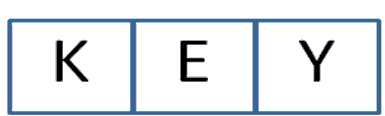
\includegraphics[width=25ex]{../latex/img/1062/1062-1.png}
\caption*{ลูกกุญแจ}
\end{subfigure}%
\begin{subfigure}{35ex}
\centering
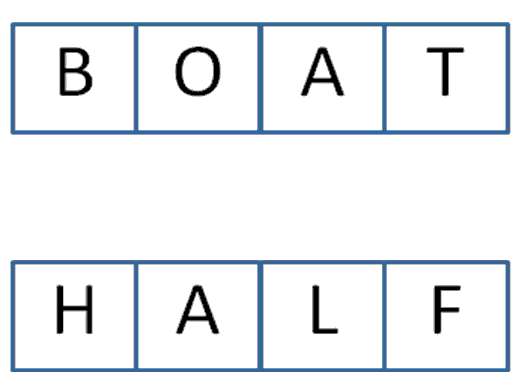
\includegraphics[width=25ex]{../latex/img/1062/1062-2.png}
\caption*{แม่กุญแจ}
\end{subfigure}%
\caption{ตัวอย่างลูกกุญแจความยาว $3$ ตัวอักษรและ แม่กุญแจความยาว $4$ ตัวอักษร}
\end{figure}

ลูกกุญแจจะเลื่อนเข้าไประหว่างแม่กุญแจ จากซ้ายไปขวา ครั้งละ $1$ ตำแหน่งตัวอักษร ในขณะที่ลูกกุญแจเลื่อนเข้าไปแต่ละครั้ง ณ ตำแหน่งแนวตั้งที่ลูกกุญแจอยู่ระหว่างแม่กุญแจจะมีตัวอักษรอยู่ $3$ ตัว ได้แก่ ตัวอักษรของลูกกุญแจส่วนที่สอดอยู่ด้านใน ($x$) ตัวอักษรของแม่กุญแจแถวบน ($a$) และแถวล่าง ($b$) สำหรับตำแหน่งแนวตั้งเหล่านั้น เราจะนำตัวอักษรทั้งสามตัวนี้มาเรียงกันตามลำดับจาก A ไปหา Z แล้วแทนค่า $x$ ในลูกกุญแจด้วยตัวอักษรกึ่งกลาง แต่จะไม่มีการเปลี่ยนแปลงตัวอักษร $a$ และ $b$

\begin{figure}[h]
\centering
\begin{subfigure}{30ex}
\centering
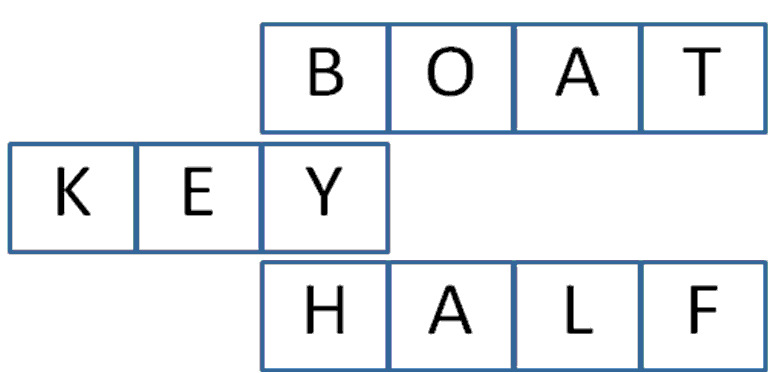
\includegraphics[width=25ex]{../latex/img/1062/1062-3.png}
\end{subfigure}%
\begin{subfigure}{20ex}
\centering
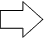
\includegraphics[width=5ex]{../latex/img/1062/1062-6.png}
\end{subfigure}%
\begin{subfigure}{30ex}
\centering
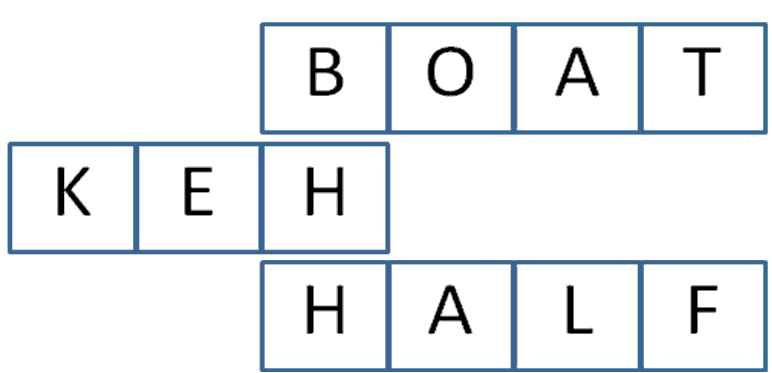
\includegraphics[width=25ex]{../latex/img/1062/1062-4.png}
\end{subfigure}%
\caption{การเปลี่ยนตัวอักษรในลูกกุญแจครั้งแรก}
\end{figure}

ในแต่ละครั้งของการเลื่อนลูกกุญแจ ถ้ามีตัวอักษรที่อยู่ระหว่างแม่กุญแจมากกว่า $1$ ตัว จะต้องดำเนินการตามเงื่อนไขข้างต้นสำหรับตัวอักษร $x$ ทุกตัว แล้วจึงเลื่อนลูกกุญแจต่อไปได้ การเลื่อนลูกกุญแจจะสิ้นสุดลงเมื่อตัวอักษรด้านซ้ายสุดของลูกกุญแจ ผ่านตัวอักษรตำแหน่งขวาสุดของแม่กุญแจไปแล้ว ดังรูปที่ 3

\begin{figure}[h!]
\centering
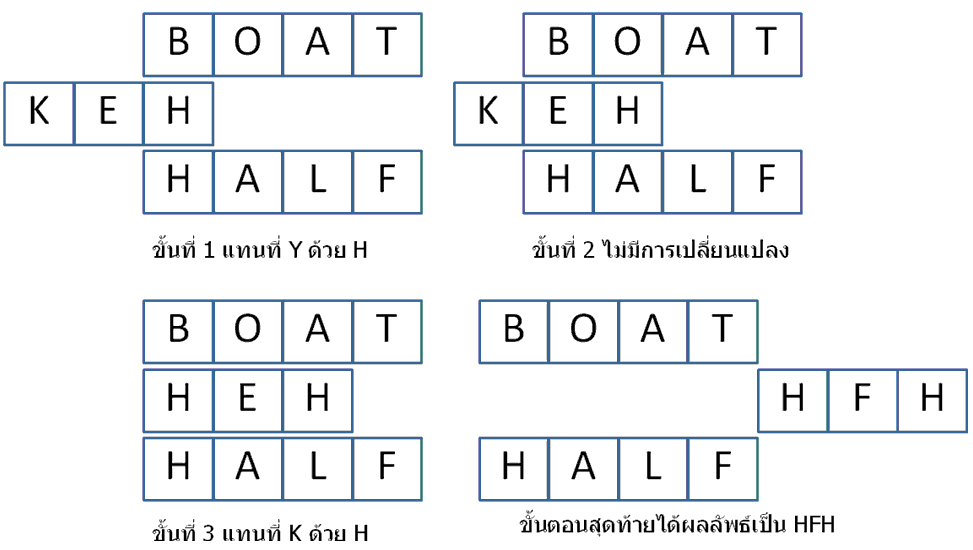
\includegraphics[width=60ex]{../latex/img/1062/1062-5.png}
\caption{ตัวอย่างการทำงานของระบบกุญแจคุโรมาตี้ครั้งที่ $1$ $2$ $3$ และ ครั้งสุดท้าย}
\end{figure}

\bigskip \newpage
\underline{\textbf{โจทย์}}  จงเขียนโปรแกรมจำลองการทำงานของกุญแจคุโรมาตี้ จากข้อมูลนำเข้าของแม่กุญแจ และลูกกุญแจแต่ละชุด พร้อมทั้งแสดงผลลัพธ์สุดท้ายของตัวอักษรที่อยู่ในลูกกุญแจ ตามลำดับจากซ้ายไปขวา

\InputFile

\textbf{บรรทัดแรก} รับข้อมูลเป็นค่าความยาวของแม่กุญแจ $L$ $(1 \leq L \leq 127)$ และค่าความยาวของลูกกุญแจ $K$ $(1 \leq K \leq 127)$ ตัวเลขทั้งสองคั่นด้วยช่องว่าง

\textbf{บรรทัดที่สองและสาม} รับข้อมูลเป็นตัวอักษรของแม่กุญแจแถวบนและล่าง ตามลำดับ มีจำนวนตัวอักษรแถวละ $L$ ตัว

\textbf{บรรทัดที่สี่} รับข้อมูลเป็นตัวอักษรของลูกกุญแจ มีจำนวน $K$ ตัว

\OutputFile

\textbf{มีบรรทัดเดียว} แสดงตัวอักษรของลูกกุญแจหลังจากสิ้นสุดกระบวนการ

\Examples

\begin{example}
\exmp{4 3
BOAT
HALF
KEY}{HFH}%
\exmp{1 4
A
Z
MAKE}{MAKE}%
\exmp{3 1
ANT
FAN
J}{N}%
\end{example}


\Source

การแข่งขันคอมพิวเตอร์โอลิมปิกสอวน.ครั้งที่ 4 ปี 2551 วันที่ 2


\end{problem}

\end{document}